\documentclass[10pt,a4paper]{article}
\usepackage[margin=1.5cm]{geometry}
\usepackage[compact]{titlesec}   % less space around section headings
\titleformat*{\section}{\large\bfseries}
\usepackage[T1]{fontenc}
\usepackage{lmodern}
\usepackage{graphicx}
\usepackage{booktabs}
\usepackage{enumitem}
\usepackage{tikz}
\usetikzlibrary{positioning}
\usepackage[hidelinks]{hyperref}

\setlist{nosep,leftmargin=*}
\setlength{\parskip}{3pt}
\setlength{\parindent}{0pt}
\setlength{\textfloatsep}{8pt}
\setlength{\intextsep}{6pt}

\title{\vspace{-1.2cm}\textbf{Live Football Analytics with a Streaming Data Pipeline}\\[2pt]
\large ID2221 Data-Intensive Computing --- Project Report, Group 28}
% TODO: check the spelling of the third surname (it was cut off in the source)
\author{Md Ahsanul Karim\\ \texttt{\small makari@kth.se}
  \and Md. Sakibul Islam\\ \texttt{\small msis3@kth.se}
  \and Singvalliyappa Velayutham\\ \texttt{\small sinvel@kth.se}}
\date{\vspace{-0.6cm}}

\begin{document}
\maketitle

\section{What we did}
We built an end-to-end streaming pipeline that turns a raw stream of football match events into a
live, minute-by-minute view of \emph{which team is on top}. Recorded matches are replayed as if they
were live: a producer sends every event to Kafka at its original timing (optionally sped up), Spark
Structured Streaming computes per-team statistics over sliding windows of match time, the results are
upserted into MongoDB, and a web dashboard receives every change through a MongoDB Change Stream and
redraws its charts within seconds. Everything runs locally with Docker Compose.

\section{Dataset}
We use \textbf{StatsBomb Open Data} (\url{https://github.com/statsbomb/open-data}), event data from the
FIFA World Cup 2022 (competition 43, season 106). Each match is a JSON list of timestamped events
(passes, pressures, shots with expected goals (xG), \dots). We use three group-stage matches: Canada--Morocco 1--2 (3\,388 events),
England--Iran 6--2 (3\,649) and Croatia--Belgium 0--0 (4\,116), 8.9\,MB in total. The data is not
included in the zip file. In \texttt{scripts/download\_statsbomb.py -{}-limit 3} downloads exactly these matches.

\section{Methodology}
\begin{figure}[!htb]
\centering
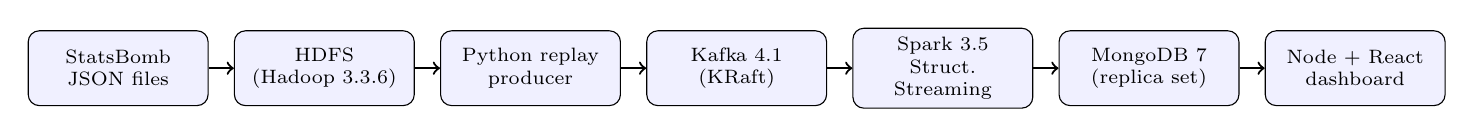
\begin{tikzpicture}[node distance=0.32cm, every node/.style={font=\scriptsize, align=center},
  box/.style={draw, rounded corners, fill=blue!6, minimum height=0.95cm, text width=2.05cm}]
\node[box] (sb) {StatsBomb\\JSON files};
\node[box, right=of sb] (hdfs) {HDFS\\(Hadoop 3.3.6)};
\node[box, right=of hdfs] (prod) {Python replay\\producer};
\node[box, right=of prod] (kafka) {Kafka 4.1\\(KRaft)};
\node[box, right=of kafka] (spark) {Spark 3.5\\Struct.\ Streaming};
\node[box, right=of spark] (mongo) {MongoDB 7\\(replica set)};
\node[box, right=of mongo] (dash) {Node + React\\dashboard};
\foreach \a/\b in {sb/hdfs, hdfs/prod, prod/kafka, kafka/spark, spark/mongo, mongo/dash}
  \draw[->, thick] (\a) -- (\b);
\end{tikzpicture}
\caption{Pipeline architecture. All components run as Docker containers on one machine.}
\end{figure}

\textbf{Storage and replay:} The raw files are stored in HDFS. The producer reads matches through
WebHDFS and sends each event to the Kafka topic \texttt{football-events}, keyed by match id so a
match stays in order within one partition. It keeps the original gaps between events, divided by a
\texttt{-{}-speed} factor, and can replay several matches concurrently. Each message carries an \emph{event time} (kickoff + elapsed match time, half-time
skipped) and the wall-clock send time \texttt{sent\_at} for latency measurement.

\textbf{Stream processing:} A PySpark Structured Streaming job (standalone cluster, one worker with
2 cores) parses the messages and counts, per match replay and team, shots, shots on target, goals,
xG, pressures and passes over \textbf{sliding event-time windows} of 5 minutes that advance every
minute. Because windows are defined on match time, the results are identical at any replay speed. We
use \emph{update} output mode, so every micro-batch emits only the windows that changed, and a
\texttt{foreachBatch} sink replaces each window's MongoDB document by its key
(\texttt{match|kickoff|team|window\_start}). This upsert is idempotent, so a batch re-run after a
failure does not double count. Spark's state and Kafka offsets are checkpointed in HDFS.

\textbf{Dashboard:} MongoDB runs as a single-node replica set because Change Streams require the
oplog. A Node.js server sends a snapshot of all windows to each browser, then pushes every change
over a WebSocket also a React client draws one line per team for each statistic (Figure~\ref{fig:dash}).

\textbf{Evaluation:} (i) \emph{Results:} \texttt{evaluation/match\_summary.py} aggregates the windows
of each match. (ii) \emph{Correctness:} we recomputed every window directly from the raw JSON and
compared it with Spark's output. (iii) \emph{Latency:} \texttt{evaluation/latency.py} watches the
Change Stream and records, for every update, the time since the producer sent the newest event in
that window (end-to-end: producer $\rightarrow$ Kafka $\rightarrow$ Spark $\rightarrow$ MongoDB
$\rightarrow$ consumer). Hardware: Apple-silicon laptop, 8\,GB RAM, 3.8\,GB for Docker.

\section{Results}
\begin{figure}[!htb]
\centering
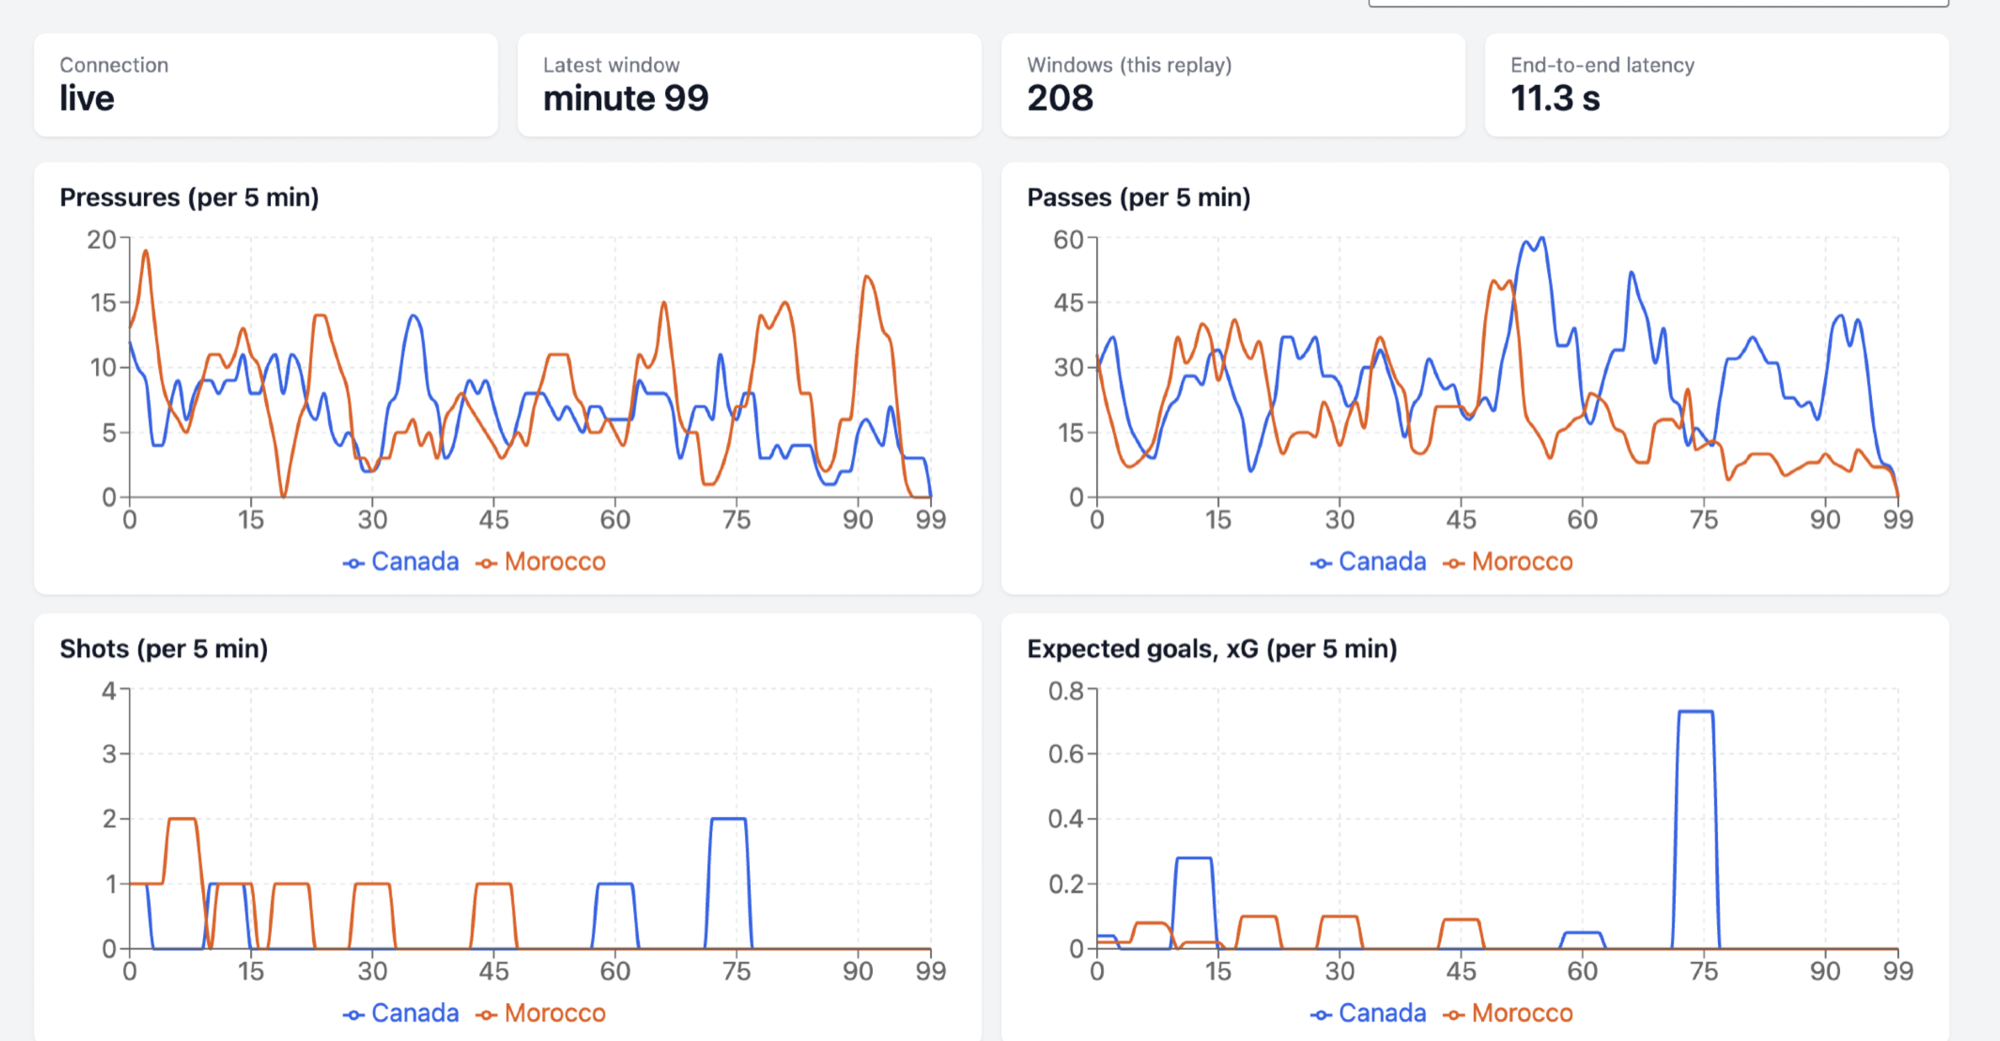
\includegraphics[width=0.6\textwidth]{figures/dashboard.png}
\caption{Live dashboard for Canada--Morocco: pressures, passes, shots and xG per team in the last
5 minutes, plotted against the match minute.}
\label{fig:dash}
\end{figure}

\textbf{Football results:} Table~\ref{tab:football} summarizes what the pipeline found.
\emph{Pressed more} is the share of match minutes in which a team made more pressures than its
opponent in the 5-minute window. In all three matches \textbf{the team with less of the ball did the
pressing}: Morocco, Croatia and Iran out-pressed their opponents in 55--66\% of the minutes, while
Canada, Belgium and England had more passes. \textbf{Creating chances is not the same as winning:}
Canada (xG 1.10 vs.\ 0.41) and Belgium (2.39 vs.\ 0.68, 16 shots) created more but did not win, while England turned an xG of 1.99 into six goals. The time series also show \emph{when} things happened (Figure~\ref{fig:dash}): Morocco pressed hardest in minutes 2--7, when they scored first while Canada dominated possession from minute 50 to 75 and had their best chance around minute 73 (xG 0.73), before Morocco's pressing rose again to close out the win.

\begin{table}[!htb]
\centering\small
\begin{tabular}{llrrrrrr}
\toprule
Match (score) & Team & Passes & Pressures & Pressed more & Shots & xG & Goals \\
\midrule
Canada--Morocco (1--2) & Canada  & \textbf{562} & 135 & 37\% & 5 & \textbf{1.10} & 0 \\
                       & Morocco & 393 & \textbf{154} & \textbf{55\%} & 7 & 0.41 & \textbf{2} \\
Belgium--Croatia (0--0) & Belgium & \textbf{630} & 119 & 27\% & \textbf{16} & \textbf{2.39} & 0 \\
                        & Croatia & 609 & \textbf{164} & \textbf{66\%} & 11 & 0.68 & 0 \\
England--Iran (6--2) & England & \textbf{846} & 101 & 28\% & \textbf{13} & \textbf{1.99} & \textbf{6} \\
                     & Iran    & 247 & \textbf{141} & \textbf{59\%} & 8 & 1.45 & 2 \\
\bottomrule
\end{tabular}
\caption{Whole-match totals computed from Spark's windows (non-overlapping windows summed).
Morocco's own goal in Canada's favour is not a Canada shot.}
\label{tab:football}
\end{table}

\textbf{Correctness:} For three matches replayed concurrently, all 653 windows matched the batch recomputation exactly (0 missing, 0 extra, 0 differing values) and two consecutive replays of the same match also matched exactly.

\textbf{Latency:} With one match, the median end-to-end latency is about 5\,s regardless of speed
(Table~\ref{tab:latency}): Spark keeps up, and latency is dominated by the fixed cost of a micro-batch
(scheduling, state checkpoint to HDFS, MongoDB write) rather than by data volume. Slower replays
give more updates (each window is rewritten in more batches), so the dashboard moves more smoothly.
Three concurrent matches double the median to 9.7\,s, since each batch must update more
windows and state on the 2-core worker.

\begin{table}[!htb]
\centering\small
\begin{tabular}{lrrrr}
\toprule
Configuration & Updates & Median & p95 & Max \\
\midrule
1 match, speed 10   & 1088 & 4.9\,s & 9.5\,s  & 16.4\,s \\
1 match, speed 60   &  362 & 5.1\,s & 10.0\,s & 13.0\,s \\
3 matches, speed 30 & 1154 & 9.7\,s & 20.7\,s & 29.7\,s \\
\bottomrule
\end{tabular}
\caption{End-to-end latency, one run per configuration (\texttt{evaluation/results.csv}).}
\label{tab:latency}
\end{table}

\textbf{Lessons learned:} (1) Replaying faster than real time makes event time run ahead of the
clock, so a new replay started ``behind'' Spark's global watermark and was dropped as late data then a
2\,h watermark (longer than any match) fixes this without delaying output in update mode.
(2) Overlapping replays of the same match were merged until the kickoff was added to the window key.
(3) \texttt{startingOffsets=latest} skips events sent before the first micro-batch.
(4) Spark's \texttt{current\_timestamp()} is fixed at batch start, so we measure latency at the
consumer. \emph{Limitations:} one run per configuration on one laptop and more workers and tuning are future work.

\section{How to run}
Requirements: Docker Desktop (about 4\,GB memory), Python 3 with \texttt{pymongo} for the evaluation
scripts. Full details are in \texttt{README.md}.
{\footnotesize
\begin{verbatim}
python3 scripts/download_statsbomb.py --limit 3     # dataset -> data/
docker compose up -d                                # HDFS, Kafka, Spark, MongoDB, dashboard
./scripts/create_topics.sh && ./scripts/upload_to_hdfs.sh
./scripts/run_spark_job.sh --reset                  # terminal 1; wait for "batch 0"
docker compose run --rm producer --speed 10         # terminal 2; no --match = all 3 matches
open http://localhost:3000                          # live dashboard
python3 evaluation/latency.py --label "1 match"     # start before the producer; Ctrl+C after
python3 evaluation/match_summary.py                 # after a replay -> match_summary.csv
\end{verbatim}
}

\end{document}
